\documentclass[twoside]{book}

\usepackage[paperwidth=148mm, paperheight=210mm]{geometry}
\usepackage{fontspec}
%\usepackage[latin1]{inputenc}
\usepackage[latin.medieval, french]{babel}
\usepackage[strict]{changepage}
\usepackage{fancyhdr}
\usepackage{paracol}
\usepackage{tableof}
\usepackage{setspace}
\usepackage{alltt}
\usepackage{titlesec}
\usepackage{xcolor}
\usepackage{xstring}
\usepackage{enumitem}

%%%%%%%%%%%%%%%%%%%%%%%%%%%%%%%%%%%%%%%%%%%%%%%%%%% Mise ne page %%%%%%%%%%%%%%%%%%%%%%%%%%%%%%
% on numérote les nbp par page et non globalement
\usepackage[perpage]{footmisc}

% définition des en-têtes et pieds de page
\pagestyle{empty}
\fancyhead{}
\fancyfoot{}
\renewcommand{\headrulewidth}{0pt}
\setlength{\headheight}{10pt}
\fancyhead[RO]{\small\thepage}
\fancyhead[LE]{\small\thepage}
% la commande titres permet de changer les titres de gauche et de droite.
\newcommand{\titres}[2]{
	\renewcommand{\rightmark}{\textcolor{red}{\sc #2}}
	\renewcommand{\leftmark}{\textcolor{red}{\sc #1}}
}
\titres{}{}

% pas d'indentation
\setlength{\parindent}{0mm}

\geometry{
inner=25mm,
outer=12mm,
top=15mm,
bottom=15mm,
headsep=3mm,
}

%%%%%%%%%%%%%%%%%%%%%%%%%%%%%%%%%%%%%%%%%%%%%%%%% Options gregorio %%%%%%%%%%%%%%%%%%%%%%%%%

\usepackage[forcecompile]{gregoriotex}
%\usepackage{gregoriotex}

%% style général de gregorio :
% lignes rouges, commenter pour du noir
\gresetlinecolor{gregoriocolor}

% texte <alt> (au-dessus de la portée) en rouge et en petit, avec réglage de sa position verticale
\grechangestyle{abovelinestext}{\color{gregoriocolor}\footnotesize}
\newcommand{\altraise}{-0.3cm}
\grechangedim{abovelinestextraise}{\altraise}{scalable}

% taille des initiales
\newcommand{\initialsize}[1]{
    \grechangestyle{initial}{\fontspec{Zallman}\fontsize{#1}{#1}\selectfont}
}
\newcommand{\defaultinitialsize}{32}
\initialsize{\defaultinitialsize}
% espace avant et après les initiales
\newcommand{\initialspace}[1]{
  \grechangedim{afterinitialshift}{#1}{scalable}
  \grechangedim{beforeinitialshift}{#1}{scalable}
}
\newcommand{\defaultinitialspace}{0cm}
\initialspace{\defaultinitialspace}


% on définit le système qui capture des headers pour générer des annotations
% cette commande sera appelée pour définir des abréviations ou autres substitutions
\newcommand{\resultat}{}
\newcommand{\abbrev}[3]{
  \IfSubStr{#1}{#2}{ \renewcommand{\resultat}{#3} }{}
}
\newcommand{\officepartannotation}[1]{
  \renewcommand{\resultat}{#1}
  \abbrev{#1}{ntro}{ {Intr.} }
  \abbrev{#1}{espo}{Resp.}
  \abbrev{#1}{ll}{All.}
  \abbrev{#1}{act}{Tract.}
  \abbrev{#1}{equen}{Seq.}
  \abbrev{#1}{ffert}{Off.}
  \abbrev{#1}{ommun}{Co.}
  \abbrev{#1}{ntip}{Ant.}
  \abbrev{#1}{ntic}{Cant.}
  \abbrev{#1}{Toni Communes}{}
  \abbrev{#1}{yrial}{}
  \greannotation{\resultat}
}
\newcommand{\modeannotation}[1]{
  \renewcommand{\resultat}{#1}
  \abbrev{#1}{1}{ {\sc i} }
  \abbrev{#1}{2}{ {\sc ii} }
  \abbrev{#1}{3}{ {\sc iii} }
  \abbrev{#1}{4}{ {\sc iv} }
  \abbrev{#1}{5}{ {\sc v} }
  \abbrev{#1}{6}{ {\sc vi} }
  \abbrev{#1}{7}{ {\sc vii} }
  \abbrev{#1}{8}{ {\sc viii} }
  \greannotation{\resultat}
}
\gresetheadercapture{office-part}{officepartannotation}{}
\gresetheadercapture{mode}{modeannotation}{string}

%%%%%%%%%%%%%%%%%%%%%%%%%%%%%%%%%%%%%%%%%%%%%% Graphisme %%%%%%%%%%%%%%%%%%%%%%%%%%%
% on définit l'échelle générale

\newcommand{\echelle}{0.85}

% on centre les titres et on ne les numérote pas
\titleformat{\section}[block]{\Large\filcenter\sc}{}{}{}
\titleformat{\subsection}[block]{\large\filcenter\sc}{}{}{}
\titleformat{\paragraph}[block]{\filcenter\sc}{}{}{}
\setcounter{secnumdepth}{0}
% on diminue l'espace avant les titres
\titlespacing*{\paragraph}{0pt}{1ex}{.6ex}

% commandes versets, repons et croix
\newcommand{\vv}{\textcolor{red}{\fontspec[Scale=\echelle]{Charis SIL}℣.\hspace{3mm}}}
\newcommand{\rr}{\textcolor{red}{\fontspec[Scale=\echelle]{Charis SIL}℟.\hspace{3mm}}}
\newcommand{\cc}{\textcolor{red}{\fontspec[Scale=\echelle]{FreeSerif}\symbol{"2720}~}}
\renewcommand{\aa}{\textcolor{red}{\fontspec[Scale=\echelle]{Charis SIL}\Abar.\hspace{3mm}}}

% commandes diverses
\newcommand{\antiphona}{\textcolor{red}{\noindent Antiphona.\hspace{4mm}}}
\newcommand{\antienne}{\textcolor{red}{\noindent Antienne.\hspace{4mm}}}
\newcommand{\rubrique}[1]{\textcolor{red}{\emph{#1}}}
\newcommand{\saut}{\\ \null \hspace{1cm}}
\newcommand{\minisaut}{\\ \null \hspace{4mm}}
\newcommand{\sautRV}{\\ \null \hspace{5.95mm}}
\newcommand{\petitvspace}{\vspace{2mm}}
\newcommand{\microvspace}{\vspace{0.8mm}}
% pour affichier 1 en rouge et un peu d'espace
\newcommand{\un}{{\color{gregoriocolor} 1~~~}}

% abréviations
\newcommand{\tpalleluia}{\rubrique{(T.P.} \mbox{Allelúia.\rubrique{)}}}
\newcommand{\tpalleluiafr}{\rubrique{(T.P.} \mbox{Alléluia.\rubrique{)}}}

\newcommand{\tqomittitur}{{\small \rubrique{(In Tempore Quadragesimæ ommittitur} Allelúia.\rubrique{)}}}
\newcommand{\careme}{{\small \rubrique{(Pendant le Carême on omet l'}Alléluia.\rubrique{)}}}

% environnement hymne : alltt + normalfont + marges custom
\newenvironment{hymne}
  {
  \begin{adjustwidth}{1.6cm}{1mm}
  \begin{alltt}\normalfont
  }
  {
  \end{alltt}
  \end{adjustwidth}
  }
  
% la commande \u permet de souligner les inflexions
\let\u\underline

% on définit la police par défaut
\setmainfont[Ligatures=TeX, Scale=\echelle]{Charis SIL}
%renderer=ICU a l'air de ne plus marcher...
%\setmainfont[Renderer=ICU, Ligatures=TeX, Scale=\echelle]{Charis SIL}
\setstretch{0.9}

% paramétrage de paracol en mode 2 colonnes par page : taille des colonnes, séparateur
\columnratio{0.5}
\setlength{\columnsep}{1.5em}
\setlength{\columnseprule}{0.3pt}

\begin{document}

% ceci est pour conserver une numérotation ordinaire malgré paracol
\twosided[pb]

\begin{titlepage}
\centering\null

\vspace{1cm}

{\scshape\LARGE Dominica III. Adventus}

~

\vspace{2cm}
{\scshape\Large Ad Matutinum}

\vspace{5cm}

{\scshape\LARGE 3\ieme~dimanche de l'Avent}

~

\vspace{2cm}
{\scshape\Large À Matines}


\vfill

{MMXXI a Matthias Bry editum}

\end{titlepage}

\null\newpage

% tolérance infinie sur les sauts de lignes pour les colonnes étroites
\sloppy

%\begin{paracol}{2}
%\vv Dómine, lábia \cc mea apéries. \\
%\rr Et os meum annuntiábit laudem tuam. \\
%\vv Deus \cc in adjutórium meum inténde. \\
%\rr Dómine, ad adjuvándum me festína. \\
%\vv Glória Patri, et Fílio, et Spirítui Sancto. \\
%\rr Sicut erat in princípio, et nunc, et semper, et in sǽcula sæculórum. Amen. Allelúia.
%\switchcolumn
%\vv Seigneur, Vous ouvrirez mes lèvres. \\
%\rr Et ma bouche annoncera Votre louange. \\
%\vv Dieu, venez à mon aide. \\
%\rr Seigneur, hâtez-vous de me secourir. \\
%\vv Gloire au Père, au Fils, et au Saint-Esprit. \\
%\rr Comme il était au commencement, maintenant et toujours, et dans les siècles des siècles. Ainsi soit-il. Alléluia.
%\end{paracol}
\gregorioscore{partitions/OA.gabc}
\section{Invitatoire}

\gregorioscore{partitions/I.gabc}

\newpage
\section{Hymne}

\gregorioscore{partitions/H.gabc}

\begin{alltt}\normalfont
          Verbe suprême
          qui sortez du sein éternel du Père,
          et qui, né dans le temps,
          venez au secours de l’univers.
          
          Illuminez en ce moment nos cœurs ;
          embrasez-les de votre amour ;
          pour que, détachés des biens périssables,
          ils soient remplis d’une joie céleste ;
          
          Afin, qu’au jour où le Juge,
          du haut de son tribunal,
          condamnera les coupables aux flammes ;
          et, d’une voix amie, conviera les bons au ciel,
          
          Nous ne soyons pas du nombre de ceux qui,
          voués à des feux éternels, seront lancés dans un noir tourbillon ;
          mais que, favorisés de la vue de Dieu,
          nous goûtions les délices du Paradis.
          
          Au Père, au Fils
          et à vous, Esprit-Saint,
          soient à jamais dans tous les siècles,
          comme il fut toujours, la gloire.
          Ainsi soit-il.
\end{alltt}

\section{Premier nocturne}

\subsection{Psaume 1}

\gregorioscore{partitions/N1A1.gabc}
\emph{\aa Voici que viendra le Roi, le Très-haut, avec une grande puissance, pour sauver les nations, alléluia.}
\newpage
\gresetinitiallines{0}
\gregorioscore{partitions/1_g.gabc}
\gresetinitiallines{1}

\begin{paracol}{2}
\begin{enumerate}[wide, itemsep=0mm, labelwidth=!, labelindent=0pt, label=\color{gregoriocolor}\theenumi]
\selectlanguage{latin}
\item Beátus vir, qui non ábiit in consílio impiórum,~† et in via pecca\textbf{tó}rum non \textbf{ste}tit,~* et in cáthedra pestilénti\textit{æ} \textit{non} \textbf{se}dit:
\item Sed in lege Dómini vo\textbf{lún}tas \textbf{e}jus,~* et in lege ejus meditábitur di\textit{e} \textit{ac} \textbf{noc}te.
\item Et erit tamquam lignum, quod plantátum est secus de\textbf{cúr}sus a\textbf{quá}rum,~* quod fructum suum dabit in tém\textit{po}\textit{re} \textbf{su}o:
\item Et fólium \textbf{e}jus non \textbf{dé}fluet:~* et ómnia quæcúmque fáciet, pro\textit{spe}\textit{ra}\textbf{bún}tur.
\item Non sic \textbf{ím}pii, \textbf{non} sic:~* sed tamquam pulvis, quem prójicit ventus a fá\textit{ci}\textit{e} \textbf{ter}ræ.
\item Ideo non resúrgent ímpii \textbf{in} ju\textbf{dí}cio:~* neque peccatóres in concíli\textit{o} \textit{jus}\textbf{tó}rum.
\item Quóniam novit Dóminus \textbf{vi}am jus\textbf{tó}rum:~* et iter impió\textit{rum} \textit{per}\textbf{í}bit.
\item Glória \textbf{Pa}tri, et \textbf{Fí}lio,~* et Spirí\textit{tu}\textit{i} \textbf{Sanc}to.
\item Sicut erat in princípio, et \textbf{nunc}, et \textbf{sem}per,~* et in sǽcula sæcu\textit{ló}\textit{rum}. \textbf{A}men.
\selectlanguage{french}
\end{enumerate}
\switchcolumn
\begin{enumerate}[wide, itemsep=0mm, labelwidth=!, labelindent=0pt, before=\itshape, label=\color{gregoriocolor}\theenumi]
\item Heureux est l'homme qui n'entre pas au conseil des méchants, + qui ne suit pas le chemin des pécheurs, * ne siège pas avec ceux qui ricanent,
\item mais se plaît dans la loi du Seigneur et murmure sa loi jour et nuit !
\item Il est comme un arbre planté près d'un ruisseau, + qui donne du fruit en son temps, * et jamais son feuillage ne meurt ; tout ce qu'il entreprend réussira,
\item tel n'est pas le sort des méchants. Mais ils sont comme la paille balayée par le vent : +
\item au jugement, les méchants ne se lèveront pas, * ni les pécheurs au rassemblement des justes.
\item Le Seigneur connaît le chemin des justes, mais le chemin des méchants se perdra.
\end{enumerate}
\end{paracol}

\subsection{Psaume 2}

\gregorioscore{partitions/N1A2.gabc}
\emph{\aa Fortifiez les mains languissantes, prenez courage et dites : Voici notre Dieu viendra et il nous sauvera, alléluia.}
\gresetinitiallines{0}
\gregorioscore{partitions/2m.gabc}
\gresetinitiallines{1}

\begin{paracol}{2}
\begin{enumerate}[wide, itemsep=0mm, labelwidth=!, labelindent=0pt, label=\color{gregoriocolor}\theenumi]
\selectlanguage{latin}
\item Quare fremuérunt \textbf{Gen}tes:~* et pópuli meditáti sunt \textit{in}\textbf{á}\textbf{ni}a?
\item Astitérunt reges terræ, et príncipes convenérunt in \textbf{u}num~* advérsus Dóminum, et advérsus Chris\textit{tum} \textbf{e}jus.
\item Dirumpámus víncula e\textbf{ó}rum:~* et projiciámus a nobis jugum \textit{ip}\textbf{só}rum.
\item Qui hábitat in cælis, irridébit \textbf{e}os:~* et Dóminus subsanná\textit{bit} \textbf{e}os.
\item Tunc loquétur ad eos in ira \textbf{su}a,~* et in furóre suo conturbá\textit{bit} \textbf{e}os.
\item Ego autem constitútus sum Rex ab eo super Sion montem sanctum \textbf{e}jus,~* prǽdicans præcép\textit{tum} \textbf{e}jus.
\item Dóminus dixit \textbf{ad} me:~* Fílius meus es tu, ego hódie gé\textit{nu}\textbf{i} te.
\item Póstula a me, et dabo tibi Gentes hereditátem \textbf{tu}am,~* et possessiónem tuam térmi\textit{nos} \textbf{ter}ræ.
\item Reges eos in virga \textbf{fér}rea,~* et tamquam vas fíguli confrín\textit{ges} \textbf{e}os.
\item Et nunc, reges, intel\textbf{lí}gite:~* erudímini, qui judicá\textit{tis} \textbf{ter}ram.
\item Servíte Dómino in ti\textbf{mó}re:~* et exsultáte ei cum \textit{tre}\textbf{mó}re.
\item Apprehéndite disciplínam, nequándo irascátur \textbf{Dó}minus,~* et pereátis de vi\textit{a} \textbf{jus}ta.
\item Cum exárserit in brevi ira \textbf{e}jus:~* beáti omnes qui confídunt \textit{in} \textbf{e}o.
\item Glória Patri, et \textbf{Fí}lio,~* et Spirítu\textit{i} \textbf{Sanc}to.
\item Sicut erat in princípio, et nunc, et \textbf{sem}per,~* et in sǽcula sæculó\textit{rum}. \textbf{A}men.
\selectlanguage{french}
\end{enumerate}
\switchcolumn
\begin{enumerate}[wide, itemsep=0mm, labelwidth=!, labelindent=0pt, before=\itshape, label=\color{gregoriocolor}\theenumi]
\item Pourquoi ce tumulte des nations, ce vain murmure des peuples ?
\item Les rois de la terre se dressent, les grands se liguent entre eux contre le Seigneur et son messie :
\item « Faisons sauter nos chaînes, rejetons ces entraves ! »
\item Celui qui règne dans les cieux s'en amuse, le Seigneur les tourne en dérision ;
\item puis il leur parle avec fureur , et sa colère les épouvante :
\item « Moi, j'ai sacré mon roi sur Sion, ma sainte montagne. »
\item Je proclame le décret du Seigneur ! + Il m'a dit : « Tu es mon fils ; moi, aujourd'hui, je t'ai engendré.
\item Demande, et je te donne en héritage les nations, pour domaine la terre tout entière.
\item Tu les détruiras de ton sceptre de fer, tu les briseras comme un vase de potier. »
\item Maintenant, rois, comprenez, reprenez-vous, juges de la terre.
\item Servez le Seigneur avec crainte, rendez-lui votre hommage en tremblant.
\item Qu'il s'irrite et vous êtes perdus : soudain sa colère éclatera. Heureux qui trouve en lui son refuge !
\end{enumerate}
\end{paracol}

\subsection{Psaume 3}

\gregorioscore{partitions/N1A3.gabc}
\emph{\aa Réjouissez-vous tous et livrez-vous à la joie, car voici que le Seigneur de la vengeance viendra, il amènera la rétribution, il viendra lui-même et nous sauvera.}
\gresetinitiallines{0}
\gregorioscore{partitions/3_si_a.gabc}
\gresetinitiallines{1}

\begin{paracol}{2}
\begin{enumerate}[wide, itemsep=0mm, labelwidth=!, labelindent=0pt, label=\color{gregoriocolor}\theenumi]
\selectlanguage{latin}
\item Dómine quid multiplicáti sunt qui \textbf{trí}bu\textbf{lant} me?~* multi in\textbf{súr}gunt ad\textbf{vér}sum me.
\item Multi dicunt \textbf{á}nimæ \textbf{me}æ:~* Non est salus ipsi in \textbf{De}o \textbf{e}jus.
\item Tu autem, Dómine, su\textbf{scép}tor \textbf{me}\textbf{us} es,~* glória mea, et exáltans \textbf{ca}put \textbf{me}um.
\item Voce mea ad Dómi\textbf{num} cla\textbf{má}vi:~* et exaudívit me de monte \textbf{sanc}to \textbf{su}o.
\item Ego dormívi, et \textbf{so}po\textbf{rá}\textbf{tus} sum:~* et exsurréxi, quia Dómi\textbf{nus} su\textbf{scé}pit me.
\item Non timébo míllia pópuli \textbf{cir}cum\textbf{dán}\textbf{tis} me:~* exsúrge, Dómine, salvum me fac, \textbf{De}us \textbf{me}us.
\item Quóniam tu percussísti omnes adversántes mihi \textbf{si}ne \textbf{cau}sa:~* dentes peccatórum \textbf{con}tri\textbf{vís}ti.
\item Dómi\textbf{ni} est \textbf{sa}lus:~* et super pópulum tuum bene\textbf{díc}tio \textbf{tu}a.
\item Glória \textbf{Pa}tri, et \textbf{Fí}\textbf{li}o,~* et Spi\textbf{rí}tui \textbf{Sanc}to.
\item Sicut erat in princípio, et \textbf{nunc}, et \textbf{sem}per,~* et in sǽcula sæcu\textbf{ló}rum. \textbf{A}men.
\selectlanguage{french}
\end{enumerate}
\switchcolumn
\begin{enumerate}[wide, itemsep=0mm, labelwidth=!, labelindent=0pt, before=\itshape, label=\color{gregoriocolor}\theenumi]
\setcounter{enumi}{1}
\item Seigneur, qu'ils sont nombreux mes adversaires, nombreux à se lever contre moi,
\item nombreux à déclarer à mon sujet : « Pour lui, pas de salut auprès de Dieu ! »
\item Mais toi, Seigneur, mon bouclier, ma gloire, tu tiens haute ma tête.
\item À pleine voix je crie vers le Seigneur ; il me répond de sa montagne sainte.
\item Et moi, je me couche et je dors ; je m'éveille : le Seigneur est mon soutien.
\item Je ne crains pas ce peuple nombreux qui me cerne et s'avance contre moi.
\item Lève-toi, Seigneur ! Sauve-moi, mon Dieu ! Tous mes ennemis, tu les frappes à la mâchoire ; les méchants, tu leur brises les dents.
\item Du Seigneur vient le salut ; vienne ta bénédiction sur ton peuple !
\end{enumerate}
\end{paracol}

\subsection{Versicule}
\begin{paracol}{2}
\vv Ex Sion spécies decóris ejus.\\
\rr Deus noster maniféste véniet.\\
\vv Pater noster... \rubrique{(secrètement)} Et ne nos indúcas in tentatiónem. \\
\rr Sed líbera nos a malo. \\
\vv Exáudi, Dómine Iesu Christe, preces servórum tuórum, et miserére nobis: Qui cum Patre et Spíritu Sancto vivis et regnas in sǽcula sæculórum.\\
\rr Amen.
\switchcolumn
\vv C’est de Sion que vient l’éclat de sa splendeur. \\
\rr Notre Dieu viendra en se manifestant.\\
\vv Notre Père... Et ne nous laissez pas succomber à la tentation. \\
\rr Mais délivrez-nous du mal. \\
\vv Exaucez, Seigneur Jésus-Christ, les prières de vos serviteurs, et ayez pitié de nous, vous qui vivez et régnez avec le Père et le Saint-Esprit, dans les siècles des siècles. \rr Ainsi soit-il.
\end{paracol}

\subsection{Première leçon}

\begin{paracol}{2}
\vv Jube, domne, benedícere. \\
\vv Benedictióne perpétua benedícat nos Pater ætérnus.\\
\rr Amen.
\switchcolumn
\vv Veuillez, Maître, bénir. \\
\vv Que le Père éternel nous bénisse d'une bénédiction perpétuelle. \\
\rr Ainsi soit-il.
\end{paracol}

\paragraph{Lecture du livre du prophète Isaïe} \rubrique{Is. 26:1-6}

En ce jour-là, ce cantique sera chanté dans le pays de Juda : Nous avons une ville forte ! Le Seigneur a mis pour sauvegarde muraille et avant-mur.
Ouvrez les portes ! Elle entrera, la nation juste, qui se garde fidèle.
Immuable en ton dessein, tu préserves la paix, la paix de qui s’appuie sur toi.
Prenez appui sur le Seigneur, à jamais, sur lui, le Seigneur, le Roc éternel.
Il a rabaissé ceux qui siégeaient dans les hauteurs, il a humilié la cité inaccessible, l’a humiliée jusqu’à terre, et lui a fait mordre la poussière.
Elle sera foulée aux pieds, sous le pied des pauvres, les pas des faibles.

\begin{paracol}{2}
\vv Tu autem, Dómine, miserére nobis. \\
\rr Deo grátias.
\switchcolumn
\vv Et vous Seigneur, ayez pitié de nous. \\
\rr Rendons grâces à Dieu.
\end{paracol}

\gregorioscore{partitions/N1R1.gabc}

\emph{\rr Voici que le Seigneur apparaîtra sur une nuée blanche.\\
\emph{*} Et avec lui des milliers de Saints ; et il portera écrit sur son vêtement et sur sa cuisse : Roi des rois, et Seigneur des seigneurs.\\
\vv Il paraîtra à la fin et il ne trompera pas ; s’il met un délai, s’il tarde, attends-le, car venant, il viendra.}
\newpage
\subsection{Deuxième leçon}

\begin{paracol}{2}
\vv Jube, domne, benedícere. \\
\vv Unigénitus Dei Fílius nos benedícere et adjuváre dignétur.\\
\rr Amen.
\switchcolumn
\vv Veuillez, Maître, bénir. \\
\vv Que le Fils unique de Dieu daigne nous bénir et nous secourir.\\
\rr Ainsi soit-il.
\end{paracol}

\rubrique{Is 26:7-10}

Il est droit, le chemin du juste ; toi qui es droit, tu aplanis le sentier du juste.
Oui, sur le chemin de tes jugements, Seigneur, nous t’espérons. Dire ton nom, faire mémoire de toi, c’est le désir de l’âme.
Mon âme, la nuit, te désire, et mon esprit, au fond de moi, te guette dès l’aurore. Quand s’exercent tes jugements sur la terre, les habitants du monde apprennent la justice.
Si l’on fait grâce au méchant, il n’apprend pas la justice ; perfide sur la terre de probité, il ne voit pas la majesté du Seigneur.

\begin{paracol}{2}
\vv Tu autem, Dómine, miserére nobis. \\
\rr Deo grátias.
\switchcolumn
\vv Et vous Seigneur, ayez pitié de nous. \\
\rr Rendons grâces à Dieu.
\end{paracol}

\gregorioscore{partitions/N1R2.gabc}

\emph{\rr Bethléhem, ville du Dieu très haut, de toi sortira le Dominateur d’Israël et sa génération est du commencement des jours de l’éternité ; et il sera glorifié au milieu du monde :\\
\emph{*} Et la paix sera dans notre terre, quand il sera venu.\\
\vv Il publiera la paix aux Nations, et sa puissance depuis une mer jusqu’à l’autre mer.}

~

\subsection{Troisième leçon}

~

\begin{paracol}{2}
\vv Jube, domne, benedícere. \\
\vv Spíritus Sancti grátia illúminet sensus et corda nostra.\\
\rr Amen.
\switchcolumn
\vv Veuillez, Maître, bénir. \\
\vv Que la grâce du Saint-Esprit illumine nos esprits et nos cœurs.\\
\rr Ainsi soit-il.
\end{paracol}

\rubrique{Is 26:11-14}

Seigneur, ta main est levée : ils ne l’aperçoivent pas ; mais ils percevront, pleins de honte, ta passion pour le peuple. En vérité, le feu les dévorera, celui que tu destines à tes ennemis !
Seigneur, tu nous assures la paix : dans toutes nos œuvres, toi-même agis pour nous.
Seigneur notre Dieu, d’autres maîtres que toi ont dominé sur nous, mais de toi seul nous faisons mémoire, de ton seul nom.
Ceux-là sont morts, ils ne revivront pas ; ce sont des ombres, ils ne se relèveront pas : voilà pourquoi tu interviens, tu les extermines, tu effaces jusqu’à leur mémoire.

\begin{paracol}{2}
\vv Tu autem, Dómine, miserére nobis. \\
\rr Deo grátias.
\switchcolumn
\vv Et vous Seigneur, ayez pitié de nous. \\
\rr Rendons grâces à Dieu.
\end{paracol}

\gregorioscore{partitions/N1R3.gabc}

\emph{\rr Celui qui doit venir viendra, et il ne tardera point, et il n’y aura plus de crainte sur nos frontières :\\
\emph{*} Parce que lui-même est notre Sauveur.\\
\vv Il laissera de côté nos iniquités, et il jettera dans le profond de la mer tous nos péchés.}

\section{Deuxième nocturne}

\subsection{Psaume 8}

\gregorioscore{partitions/N2A1.gabc}
\emph{\aa Réjouis-toi et livre-toi à la joie, fille de Jérusalem ; voici que ton Roi vient à toi ; Sion, ne crains pas, car ton salut viendra bientôt.}
\gresetinitiallines{0}
\gregorioscore{partitions/4_la_E.gabc}
\gresetinitiallines{1}


\begin{paracol}{2}

\begin{enumerate}[wide, itemsep=0mm, labelwidth=!, labelindent=0pt, label=\color{gregoriocolor}\theenumi]
\selectlanguage{latin}
\item Dómine, Dó\textit{mi}\textit{nus} \textbf{nos}ter,~* quam admirábile est nomen tuum in u\textit{ni}\textit{vér}\textit{sa} \textbf{ter}ra!
\item Quóniam eleváta est magnificén\textit{ti}\textit{a} \textbf{tu}a,~* \textit{su}\textit{per} \textbf{cæ}los.
\item Ex ore infántium et lacténtium perfecísti laudem propter ini\textit{mí}\textit{cos} \textbf{tu}os,~* ut déstruas inimí\textit{cum} \textit{et} \textit{ul}\textbf{tó}rem.
\item Quóniam vidébo cælos tuos, ópera digitó\textit{rum} \textit{tu}\textbf{ó}rum:~* lunam et stellas, \textit{quæ} \textit{tu} \textit{fun}\textbf{dás}ti.
\item Quid est homo quod me\textit{mor} \textit{es} \textbf{e}jus?~* aut fílius hóminis, quóniam \textit{ví}\textit{si}\textit{tas} \textbf{e}um?
\item Minuísti eum paulo minus ab Angelis,~† glória et honóre coro\textit{nás}\textit{ti} \textbf{e}um:~* et constituísti eum super ópera má\textit{nu}\textit{um} \textit{tu}\textbf{á}rum.
\item Omnia subjecísti sub pé\textit{di}\textit{bus} \textbf{e}jus,~* oves et boves univérsas: ínsuper et \textit{pé}\textit{co}\textit{ra} \textbf{cam}pi.
\item Vólucres cæli, et \textit{pi}\textit{sces} \textbf{ma}ris,~* qui perámbulant \textit{sé}\textit{mi}\textit{tas} \textbf{ma}ris.
\item Dómine, Dó\textit{mi}\textit{nus} \textbf{nos}ter,~* quam admirábile est nomen tuum in u\textit{ni}\textit{vér}\textit{sa} \textbf{ter}ra!
\item Glória Pa\textit{tri}, \textit{et} \textbf{Fí}lio,~* et Spi\textit{rí}\textit{tu}\textit{i} \textbf{Sanc}to.
\item Sicut erat in princípio, et \textit{nunc}, \textit{et} \textbf{sem}per,~* et in sǽcula sæ\textit{cu}\textit{ló}\textit{rum}. \textbf{A}men.
\selectlanguage{french}
\end{enumerate}

\switchcolumn
\begin{enumerate}[wide, itemsep=0mm, labelwidth=!, labelindent=0pt, before=\itshape, label=\color{gregoriocolor}\theenumi]
\setcounter{enumi}{1}
\item Ô Seigneur, notre Dieu, qu'il est grand ton nom par toute la terre ! Jusqu'aux cieux, ta splendeur est chantée
\item par la bouche des enfants, des tout-petits : rempart que tu opposes à l'adversaire, où l'ennemi se brise en sa révolte.
\item À voir ton ciel, ouvrage de tes doigts, la lune et les étoiles que tu fixas,
\item qu'est-ce que l'homme pour que tu penses à lui, le fils d'un homme, que tu en prennes souci ?
\item Tu l'as voulu un peu moindre qu'un dieu, le couronnant de gloire et d'honneur ;
\item tu l'établis sur les oeuvres de tes mains, tu mets toute chose à ses pieds :
\item les troupeaux de boeufs et de brebis, et même les bêtes sauvages,
\item les oiseaux du ciel et les poissons de la mer, tout ce qui va son chemin dans les eaux.
\item Ô Seigneur, notre Dieu, qu'il est grand ton nom par toute la terre !
\end{enumerate}

\end{paracol}

\subsection{Psaume 9-1}

\gregorioscore{partitions/N2A2.gabc}
\emph{\aa Notre Roi, le Christ, viendra, lui que Jean a prédit être l’Agneau qui doit venir.}
\gresetinitiallines{0}
\gregorioscore{partitions/5.gabc}
\gresetinitiallines{1}

\begin{paracol}{2}
\begin{enumerate}[wide, itemsep=0mm, labelwidth=!, labelindent=0pt, label=\color{gregoriocolor}\theenumi]
\selectlanguage{latin}
\item Confitébor tibi, Dómine, in toto corde \textbf{me}o:~* narrábo ómnia mira\textbf{bí}lia \textbf{tu}a.
\item Lætábor et exsultábo \textbf{in} te:~* psallam nómini \textbf{tu}o, Al\textbf{tís}sime.
\item In converténdo inimícum meum re\textbf{trór}sum:~* infirmabúntur, et períbunt a \textbf{fá}cie \textbf{tu}a.
\item Quóniam fecísti judícium meum et causam \textbf{me}am:~* sedísti super thronum, qui júdi\textbf{cas} jus\textbf{tí}tiam.
\item Increpásti Gentes, et périit \textbf{ím}pius:~* nomen eórum delésti in ætérnum, et in \textbf{sǽ}culum \textbf{sǽ}culi.
\item Inimíci defecérunt frámeæ in \textbf{fi}nem:~* et civitátes eórum \textbf{de}stru\textbf{xís}ti.
\item Périit memória eórum cum \textbf{só}nitu:~* et Dóminus in æ\textbf{tér}num \textbf{pér}manet.
\item Parávit in judício thronum \textbf{su}um:~* et ipse judicábit orbem terræ in æquitáte, judicábit pópulos \textbf{in} jus\textbf{tí}tia.
\item Et factus est Dóminus refúgium \textbf{páu}peri:~* adjútor in opportunitátibus, in tribu\textbf{la}ti\textbf{ó}ne.
\item Et sperent in te qui novérunt nomen \textbf{tu}um:~* quóniam non dereliquísti quæ\textbf{rén}tes te, \textbf{Dó}mine.
\item Glória Patri, et \textbf{Fí}lio,~* et Spi\textbf{rí}tui \textbf{Sanc}to.
\item Sicut erat in princípio, et nunc, et \textbf{sem}per,~* et in sǽcula sæcu\textbf{ló}rum. \textbf{A}men.
\selectlanguage{french}
\end{enumerate}
\switchcolumn
\begin{enumerate}[wide, itemsep=0mm, labelwidth=!, labelindent=0pt, before=\itshape, label=\color{gregoriocolor}\theenumi]
\setcounter{enumi}{1}
\item De tout mon coeur, Seigneur, je rendrai grâce, je dirai tes innombrables merveilles ;
\item pour toi, j'exulterai, je danserai, je fêterai ton nom, Dieu Très-Haut.
\item Mes ennemis ont battu en retraite, devant ta face, ils s'écroulent et périssent.
\item Tu as plaidé mon droit et ma cause, tu as siégé, tu as jugé avec justice.
\item Tu menaces les nations, tu fais périr les méchants, à tout jamais tu effaces leur nom.
\item L'ennemi est achevé, ruiné pour toujours, tu as rasé des villes, leur souvenir a péri.
\item Mais il siège, le Seigneur, à jamais : pour juger, il affermit son trône ;
\item il juge le monde avec justice et gouverne les peuples avec droiture.
\item Qu'il soit la forteresse de l'opprimé, sa forteresse aux heures d'angoisse :
\item ils s'appuieront sur toi, ceux qui connaissent ton nom ; jamais tu n'abandonnes, Seigneur, ceux qui te cherchent.
\end{enumerate}
\end{paracol}

\subsection{Psaume 9-2}

\gregorioscore{partitions/N2A3.gabc}
\emph{\aa Voici que je viens bientôt, et ma récompense est avec moi, dit le Seigneur ; c’est de donner à chacun selon ses œuvres.}
\gresetinitiallines{0}
\gregorioscore{partitions/6.gabc}
\gresetinitiallines{1}

\begin{paracol}{2}

\begin{enumerate}[wide, itemsep=0mm, labelwidth=!, labelindent=0pt, label=\color{gregoriocolor}\theenumi]
\selectlanguage{latin}
\item Psállite Dómino, qui hábi\textbf{tat} in \textbf{Si}on:~* annuntiáte inter Gentes stú\textit{di}\textit{a} \textbf{e}jus:
\item Quóniam requírens sánguinem eórum \textbf{re}cor\textbf{dá}tus est:~* non est oblítus cla\textit{mó}\textit{rem} \textbf{páu}perum.
\item Miserére \textbf{me}i, \textbf{Dó}mine:~* vide humilitátem meam de ini\textit{mí}\textit{cis} \textbf{me}is.
\item Qui exáltas me de \textbf{por}tis \textbf{mor}tis,~* ut annúntiem omnes laudatiónes tuas in portis fí\textit{li}\textit{æ} \textbf{Si}on.
\item Exsultábo in salu\textbf{tá}ri \textbf{tu}o:~* infíxæ sunt Gentes in intéritu, \textit{quem} \textit{fe}\textbf{cé}runt.
\item In láqueo isto, quem \textbf{abs}con\textbf{dé}runt,~* comprehénsus est \textit{pes} \textit{e}\textbf{ó}rum.
\item Cognoscétur Dóminus ju\textbf{dí}cia \textbf{fá}ciens:~* in opéribus mánuum suárum comprehénsus \textit{est} \textit{pec}\textbf{cá}tor.
\item Convertántur peccatóres \textbf{in} in\textbf{fér}num,~* omnes Gentes quæ oblivis\textit{cún}\textit{tur} \textbf{De}um.
\item Quóniam non in finem oblívio \textbf{e}rit \textbf{páu}peris:~* patiéntia páuperum non perí\textit{bit} \textit{in} \textbf{fi}nem.
\item Exsúrge, Dómine, non confor\textbf{té}tur \textbf{ho}mo:~* judicéntur Gentes in con\textit{spéc}\textit{tu} \textbf{tu}o.
\item Constítue, Dómine, legislatórem \textbf{su}per \textbf{e}os:~* ut sciant Gentes quóniam \textit{hó}\textit{mi}\textbf{nes} sunt.
\item Glória \textbf{Pa}tri, et \textbf{Fí}lio,~* et Spirí\textit{tu}\textit{i} \textbf{Sanc}to.
\item Sicut erat in princípio, et \textbf{nunc}, et \textbf{sem}per,~* et in sǽcula sæcu\textit{ló}\textit{rum}. \textbf{A}men.
\selectlanguage{french}
\end{enumerate}

\switchcolumn
\begin{enumerate}[wide, itemsep=0mm, labelwidth=!, labelindent=0pt, before=\itshape, label=\color{gregoriocolor}\theenumi]
\setcounter{enumi}{11}
\item Fêtez le Seigneur qui siège dans Sion, annoncez parmi les peuples ses exploits !
\item Attentif au sang versé, il se rappelle, il n'oublie pas le cri des malheureux.
\item Pitié pour moi, Seigneur, vois le mal que m'ont fait mes adversaires, * toi qui m'arraches aux portes de la mort ;
\item et je dirai tes innombrables louanges aux portes de Sion, * je danserai de joie pour ta victoire.
\item Ils sont tombés, les païens, dans la fosse qu'ils creusaient ; aux filets qu'ils ont tendus, leurs pieds se sont pris.
\item Le Seigneur s'est fait connaître : il a rendu le jugement, il prend les méchants à leur piège.
\item Que les méchants retournent chez les morts, toutes les nations qui oublient le vrai Dieu !
\item Mais le pauvre n'est pas oublié pour toujours : jamais ne périt l'espoir des malheureux.
\item Lève-toi, Seigneur : qu'un mortel ne soit pas le plus fort, que les nations soient jugées devant ta face !
\item Frappe-les d'épouvante, Seigneur : que les nations se reconnaissent mortelles !
\end{enumerate}

\end{paracol}

\subsection{Versicule}
\begin{paracol}{2}
\vv Emítte Agnum, Dómine, Dominatórem terræ.\\
\rr De Petra desérti ad montem fíliæ Sion.\\
\vv Pater noster... \rubrique{(secrètement)} Et ne nos indúcas in tentatiónem. \\
\rr Sed líbera nos a malo. \\
\vv Ipsíus píetas et misericórdia nos ádiuvet, qui cum Patre et Spíritu Sancto vivit et regnat in sǽcula sæculórum. \rr Amen.
\switchcolumn
\vv Envoyez, Seigneur, l’Agneau dominateur de la terre.\\
\rr De la pierre du désert à la montagne de la fille de Sion.\\
\vv Notre Père... Et ne nous laissez pas succomber à la tentation. \\
\rr Mais délivrez-nous du mal. \\
\vv Qu'il nous secoure par sa bonté et sa miséricorde, celui qui, avec le Père et le Saint-Esprit, vit et règne dans les siècles des siècles. \rr Ainsi soit-il.
\end{paracol}
\newpage
\subsection{Quatrième leçon}

\begin{paracol}{2}
\vv Jube, domne, benedícere. \\
\vv Deus Pater omnípotens sit nobis propítius et clemens.
\rr Amen.
\switchcolumn
\vv Veuillez, Maître, bénir. \\
\vv Que Dieu le Père tout-puissant soit pour nous propice et plein de clémence.
\rr Ainsi soit-il.
\end{paracol}

\paragraph{Sermon de saint Léon, Pape.}

Nous vous avertissons publiquement, mes très chers frères, et avec une sollicitude pastorale d’observer le jeûne du dixième mois. Le temps où nous sommes et la coutume de notre dévotion nous y engagent. Par ce jeûne, qu’on célèbre lorsque la récolte de tous les fruits de la terre est terminée, on offre à Dieu, qui nous a donné ces fruits, un très juste sacrifice de continence. En effet, que peut-il y avoir de plus utile que le jeûne ? Par son observance, nous nous approchons de Dieu, et, résistant au démon, nous surmontons les attraits des vices.

\begin{paracol}{2}
\vv Tu autem, Dómine, miserére nobis. \\
\rr Deo grátias.
\switchcolumn
\vv Et vous Seigneur, ayez pitié de nous. \\
\rr Rendons grâces à Dieu.
\end{paracol}

\gregorioscore{partitions/N2R1.gabc}

\emph{\rr Égypte, ne pleure pas, car ton Dominateur, en présence duquel les abîmes seront ébranlés, viendra à toi, \\
\emph{*} Pour délivrer son peuple de la main et du pouvoir de ses ennemis.\\
\vv Voici que viendra le Seigneur des armées, ton Dieu viendra avec une grande puissance.}

\newpage
\subsection{Cinquième leçon}

\begin{paracol}{2}
\vv Jube, domne, benedícere. \\
\vv Christus perpétuæ det nobis gáudia vitæ.
\rr Amen.
\switchcolumn
\vv Veuillez, Maître, bénir. \\
\vv Que le Christ nous donne les joies de l'éternelle vie.
\rr Ainsi soit-il.
\end{paracol}

Le jeûne a toujours été un aliment pour la vertu. L’abstinence produit les pensées chastes, les résolutions sages, les conseils salutaires ; et, par les mortifications volontaires, la chair meurt à ses convoitises, tandis que l’esprit reçoit une nouvelle vigueur pour pratiquer les vertus. Mais, parce que le salut de nos âmes ne s’acquiert pas uniquement par le jeûne, ajoutons au jeûne, des œuvres de miséricorde envers les pauvres. Faisons servir à la vertu ce que nous retranchons à la sensualité, et que l’abstinence de celui qui jeûne devienne le repas du pauvre.

\begin{paracol}{2}
\vv Tu autem, Dómine, miserére nobis. \\
\rr Deo grátias.
\switchcolumn
\vv Et vous Seigneur, ayez pitié de nous. \\
\rr Rendons grâces à Dieu.
\end{paracol}

\gregorioscore{partitions/N2R2.gabc}


\emph{\rr Près de venir est son temps, et ses jours ne seront pas différés :\\
\emph{*} Car le Seigneur aura pitié de Jacob, et Israël sera sauvé.\\
\vv Retourne, vierge d’Israël, retourne vers ces cités tiennes.}

\newpage
\subsection{Sixième leçon}

\begin{paracol}{2}
\vv Jube, domne, benedícere. \\
\vv Ignem sui amóris accéndat Deus in córdibus nostris.\\
\rr Amen.
\switchcolumn
\vv Veuillez, Maître, bénir. \\
\vv Que Dieu daigne allumer dans nos cœurs le feu de son amour. \\
\rr Ainsi soit-il.
\end{paracol}

Appliquons-nous à la défense des veuves, à l’assistance des orphelins, à la consolation de ceux qui pleurent : occupons-nous de pacifier ceux qui se querellent. Que l’étranger reçoive l’hospitalité ; secourons l’opprimé, donnons des vêtements à ceux qui sont nus ; environnons le malade de nos soins et de nos sollicitudes ; pour que tous ceux d’entre nous qui, par ces bonnes œuvres, auront offert à Dieu, l’auteur de tous les biens, un sacrifice de piété, méritent de recevoir de lui, en récompense, le royaume des cieux. Jeûnons donc mercredi et vendredi prochains ; et samedi, veillons ensemble dans l’église du bienheureux Apôtre saint Pierre, afin qu’aidés du suffrage de ses mérites, nous puissions obtenir ce que nous demandons, par notre Seigneur Jésus-Christ, qui vit et règne avec le Père et le Saint-Esprit, dans les siècles des siècles. Amen.

\begin{paracol}{2}
\vv Tu autem, Dómine, miserére nobis. \\
\rr Deo grátias.
\switchcolumn
\vv Et vous Seigneur, ayez pitié de nous. \\
\rr Rendons grâces à Dieu.
\end{paracol}

\gregorioscore{partitions/N2R3.gabc}

\emph{\rr Le Seigneur descendra comme la pluie sur une toison :\\
\emph{*} Dans ses jours s’élèvera la justice et une abondance de paix.\\
\vv Et tous les rois de la terre l’adoreront, toutes les nations le serviront.}

\section{Troisième nocturne}

\subsection{Psaume 9-3}

\gregorioscore{partitions/N3A1.gabc}
\emph{\aa L’Ange Gabriel parla à Marie, disant : Je vous salue, pleine de grâce, le Seigneur est avec vous, vous êtes bénie entre les femmes.}
\gresetinitiallines{0}
\gregorioscore{partitions/7_d.gabc}
\gresetinitiallines{1}

\begin{paracol}{2}

\begin{enumerate}[wide, itemsep=0mm, labelwidth=!, labelindent=0pt, label=\color{gregoriocolor}\theenumi]
\selectlanguage{latin}
\item Ut quid, Dómine, reces\textbf{sís}ti \textbf{lon}ge,~* déspicis in opportunitátibus, in tribu\textbf{la}ti\textbf{ó}ne?
\item Dum supérbit ímpius, in\textbf{cén}ditur \textbf{pau}per:~* comprehendúntur in consíliis \textbf{qui}bus \textbf{có}gitant.
\item Quóniam laudátur peccátor in desidériis \textbf{á}nimæ \textbf{su}æ:~* et iníquus \textbf{be}ne\textbf{dí}citur.
\item Exacerbávit Dómi\textbf{num} pec\textbf{cá}tor,~* secúndum multitúdinem iræ \textbf{su}æ non \textbf{quæ}ret.
\item Non est Deus in con\textbf{spéc}tu \textbf{e}jus:~* inquinátæ sunt viæ illíus in \textbf{om}ni \textbf{tém}pore.
\item Auferúntur judícia tua a \textbf{fá}cie \textbf{e}jus:~* ómnium inimicórum suórum \textbf{do}mi\textbf{ná}bitur.
\item Dixit enim in \textbf{cor}de \textbf{su}o:~* Non movébor a generatióne in generatiónem \textbf{si}ne \textbf{ma}lo.
\item Cujus maledictióne os plenum est, et amaritúdi\textbf{ne}, et \textbf{do}lo:~* sub lingua ejus \textbf{la}bor et \textbf{do}lor.
\item Sedet in insídiis cum divítibus \textbf{in} oc\textbf{cúl}tis:~* ut interfíciat \textbf{in}no\textbf{cén}tem.
\item Oculi ejus in páupe\textbf{rem} re\textbf{spí}ciunt:~* insidiátur in abscóndito, quasi leo in spe\textbf{lún}ca \textbf{su}a.
\item Insidiátur ut \textbf{rá}piat \textbf{páu}perem:~* rápere páuperem, dum \textbf{át}trahit \textbf{e}um.
\item In láqueo suo humili\textbf{á}bit \textbf{e}um:~* inclinábit se, et cadet, cum dominátus \textbf{fú}erit \textbf{páu}perum.
\item Dixit enim in corde suo: Ob\textbf{lí}tus est \textbf{De}us,~* avértit fáciem suam ne víde\textbf{at} in \textbf{fi}nem.
\item Glória \textbf{Pa}tri, et \textbf{Fí}lio,~* et Spi\textbf{rí}tui \textbf{Sanc}to.
\item Sicut erat in princípio, et \textbf{nunc}, et \textbf{sem}per,~* et in sǽcula sæcu\textbf{ló}rum. \textbf{A}men.
\selectlanguage{french}
\end{enumerate}

\switchcolumn
\begin{enumerate}[wide, itemsep=0mm, labelwidth=!, labelindent=0pt, before=\itshape, label=\color{gregoriocolor}\theenumi]
\item Pourquoi, Seigneur, es-tu si loin ? Pourquoi te cacher aux jours d'angoisse ?
\item L'impie, dans son orgueil, poursuit les malheureux : ils se font prendre aux ruses qu'il invente.
\item L'impie se glorifie du désir de son âme, l'arrogant blasphème, il brave le Seigneur ;
\item plein de suffisance, l'impie ne cherche plus : « Dieu n'est rien », voilà toute sa ruse.
\item A tout moment, ce qu'il fait réussit ; + tes sentences le dominent de très haut. * (Tous ses adversaires, il les méprise.)
\item Il s'est dit : « Rien ne peut m'ébranler, je suis pour longtemps à l'abri du malheur. »
\item Sa bouche qui maudit n'est que fraude et violence, sa langue, mensonge et blessure.
\item Il se tient à l'affût près des villages, il se cache pour tuer l'innocent. Des yeux, il épie le faible,
\item il se cache à l'affût, comme un lion dans son fourré ; il se tient à l'affût pour surprendre le pauvre, il attire le pauvre, il le prend dans son filet.
\item Il se baisse, il se tapit ; de tout son poids, il tombe sur le faible.
\item Il dit en lui-même : « Dieu oublie ! il couvre sa face, jamais il ne verra ! »
\end{enumerate}

\end{paracol}

\subsection{Psaume 9-4}

\gregorioscore{partitions/N3A2.gabc}
\emph{\aa Marie dit : Quelle pensez-vous que soit cette salutation ? Parce que mon âme a été troublée, et que je dois enfanter un Roi qui ne violera pas ma virginité.}
\gresetinitiallines{0}
\gregorioscore{partitions/8_G.gabc}
\gresetinitiallines{1}

\begin{paracol}{2}

\begin{enumerate}[wide, itemsep=0mm, labelwidth=!, labelindent=0pt, label=\color{gregoriocolor}\theenumi]
\selectlanguage{latin}
\item Exsúrge, Dómine Deus, exaltétur manus \textbf{tu}a:~* ne oblivis\textit{cá}\textit{ris} \textbf{páu}perum.
\item Propter quid irritávit ímpius \textbf{De}um?~* dixit enim in corde suo: \textit{Non} \textit{re}\textbf{quí}ret.
\item Vides quóniam tu labórem et dolórem con\textbf{sí}deras:~* ut tradas eos in \textit{ma}\textit{nus} \textbf{tu}as.
\item Tibi derelíctus est \textbf{pau}per:~* órphano tu e\textit{ris} \textit{ad}\textbf{jú}tor.
\item Cóntere bráchium peccatóris et ma\textbf{lí}gni:~* quærétur peccátum illíus, et non in\textit{ve}\textit{ni}\textbf{é}tur.
\item Dóminus regnábit in ætérnum, et in sǽculum \textbf{sǽ}culi:~* períbitis, Gentes, de ter\textit{ra} \textit{il}\textbf{lí}us.
\item Desidérium páuperum exaudívit \textbf{Dó}minus:~* præparatiónem cordis eórum audívit \textit{au}\textit{ris} \textbf{tu}a.
\item Judicáre pupíllo et \textbf{hú}mili,~* ut non appónat ultra magnificáre se homo \textit{su}\textit{per} \textbf{ter}ram.
\item Glória Patri, et \textbf{Fí}lio,~* et Spirí\textit{tu}\textit{i} \textbf{Sanc}to.
\item Sicut erat in princípio, et nunc, et \textbf{sem}per,~* et in sǽcula sæcu\textit{ló}\textit{rum}. \textbf{A}men.
\selectlanguage{french}
\end{enumerate}

\switchcolumn
\begin{enumerate}[wide, itemsep=0mm, labelwidth=!, labelindent=0pt, before=\itshape, label=\color{gregoriocolor}\theenumi]
\setcounter{enumi}{11}
\item Lève-toi, Seigneur ! Dieu, étends la main ! N'oublie pas le pauvre !
\item Pourquoi l'impie brave-t-il le Seigneur en lui disant : « Viendras-tu me cher\-cher~?~»
\item Mais tu as vu : tu regardes le mal et la souffrance, tu les prends dans ta main ; sur toi repose le faible, c'est toi qui viens en aide à l'orphelin.
\item Brise le bras de l'impie, du méchant ; alors tu chercheras son impiété sans la trouver.
\item A tout jamais, le Seigneur est roi : les païens ont péri sur sa terre.
\item Tu entends, Seigneur, le désir des pauvres, tu rassures leur coeur, tu les écoutes.
\item Que justice soit rendue à l'orphelin, qu'il n'y ait plus d'opprimé, * et que tremble le mortel, né de la terre !
\end{enumerate}

\end{paracol}

\subsection{Psaume 10}

\gregorioscore{partitions/N3A3.gabc}
\emph{\aa En l’avènement du souverain Roi, que les cœurs des hommes soient purifiés afin que nous marchions à sa rencontre d’une manière digne : car voici qu’Il vient et Il ne tardera pas.}
\gresetinitiallines{0}
\gregorioscore{partitions/4_la_E.gabc}
\gresetinitiallines{1}

\begin{paracol}{2}

\begin{enumerate}[wide, itemsep=0mm, labelwidth=!, labelindent=0pt, label=\color{gregoriocolor}\theenumi]
\selectlanguage{latin}
\item In Dómino confído:~† quómodo dícitis á\textit{ni}\textit{mæ} \textbf{me}æ:~* Tránsmigra in mon\textit{tem} \textit{sic}\textit{ut} \textbf{pas}ser?
\item Quóniam ecce peccatóres intendérunt arcum,~† paravérunt sagíttas su\textit{as} \textit{in} \textbf{phá}retra,~* ut sagíttent in obscú\textit{ro} \textit{rec}\textit{tos} \textbf{cor}de.
\item Quóniam quæ perfecísti, \textit{de}\textit{stru}\textbf{xé}runt:~* justus \textit{au}\textit{tem} \textit{quid} \textbf{fe}cit?
\item Dóminus in templo \textit{sanc}\textit{to} \textbf{su}o,~* Dóminus in cæ\textit{lo} \textit{se}\textit{des} \textbf{e}jus.
\item Oculi ejus in páupe\textit{rem} \textit{re}\textbf{spí}ciunt:~* pálpebræ ejus intérrogant \textit{fí}\textit{li}\textit{os} \textbf{hó}\textbf{mi}num.
\item Dóminus intérrogat jus\textit{tum} \textit{et} \textbf{ím}pium:~* qui autem díligit iniquitátem, odit \textit{á}\textit{ni}\textit{mam} \textbf{su}am.
\item Pluet super pecca\textit{tó}\textit{res} \textbf{lá}queos:~* ignis, et sulphur, et spíritus procellárum pars cá\textit{li}\textit{cis} \textit{e}\textbf{ó}rum.
\item Quóniam justus Dóminus, et justíti\textit{as} \textit{di}\textbf{lé}xit:~* æquitátem vi\textit{dit} \textit{vul}\textit{tus} \textbf{e}jus.
\item Glória Pa\textit{tri}, \textit{et} \textbf{Fí}lio,~* et Spi\textit{rí}\textit{tu}\textit{i} \textbf{Sanc}to.
\item Sicut erat in princípio, et \textit{nunc}, \textit{et} \textbf{sem}per,~* et in sǽcula sæ\textit{cu}\textit{ló}\textit{rum}. \textbf{A}men.
\selectlanguage{french}
\end{enumerate}

\switchcolumn
\begin{enumerate}[wide, itemsep=0mm, labelwidth=!, labelindent=0pt, before=\itshape, label=\color{gregoriocolor}\theenumi]
\setcounter{enumi}{1}
\item Auprès du Seigneur j'ai mon refuge. + Comment pouvez-vous me dire : Oiseaux, fuyez à la montagne !
\item Voici que les méchants tendent l'arc : + ils ajustent leur flèche à la corde pour viser dans l'ombre l'homme au coeur droit.
\item Quand sont ruinées les fondations, que peut faire le juste ?
\item Mais le Seigneur, dans son temple saint, + le Seigneur, dans les cieux où il trône, garde les yeux ouverts sur le monde. Il voit, il scrute les hommes ; +
\item le Seigneur a scruté le juste et le méchant : l'ami de la violence, il le hait.
\item Il fera pleuvoir ses fléaux sur les méchants, + feu et soufre et vent de tempête ; c'est la coupe qu'ils auront en partage.
\item Vraiment, le Seigneur est juste ; + il aime toute justice : les hommes droits le verront face à face.
\end{enumerate}

\end{paracol}

\subsection{Versicule}
\begin{paracol}{2}
\vv Egrediétur Dóminus de loco sancto suo.\\
\rr Véniet ut salvet pópulum suum.\\
\vv Pater noster... \rubrique{(secrètement)} Et ne nos indúcas in tentatiónem. \\
\rr Sed líbera nos a malo. \\
\vv A vínculis peccatórum nostrórum absólvat nos omnípotens et miséricors Dóminus. \rr Amen.
\switchcolumn
\vv Le Seigneur sortira de son lieu saint.\\
\rr Il viendra pour sauver son peuple.\\
\vv Notre Père... Et ne nous laissez pas succomber à la tentation. \\
\rr Mais délivrez-nous du mal. \\
\vv Que le Dieu tout-puissant et miséricordieux daigne nous délivrer des liens de nos péchés. \rr Ainsi soit-il.
\end{paracol}

\subsection{Septième leçon}

\begin{paracol}{2}
\vv Jube, domne, benedícere. \\
\vv Evangélica léctio sit nobis salus et protéctio.
\rr Amen.
\switchcolumn
\vv Veuillez, Maître, bénir. \\
\vv Que la lecture du saint Evangile nous soit salut et protection. 
\rr Ainsi soit-il.
\end{paracol}

\paragraph{Lecture du saint \'Evangile selon saint Jean} \rubrique{Jn 1 : 19-20}

Voici le témoignage de Jean, quand les Juifs lui envoyèrent de Jérusalem des prêtres et des lévites pour lui demander : « Qui es-tu ? »
Il ne refusa pas de répondre, il déclara ouvertement : « Je ne suis pas le Christ. »

\paragraph{Homélie de saint Grégoire, Pape.}

Les paroles qu’on vient de nous lire, mes très chers frères, portent notre attention sur l’humilité de saint Jean. Lui, dont la vertu était si grande qu’on avait pu croire qu’il était le Christ, il préféra demeurer simplement et inébranlablement en son propre rôle et ne pas être vainement élevé dans l’opinion des hommes au-dessus de lui-même. Car il le déclara et ne le nia point ; il le proclama : « Je ne suis pas, moi, le Christ. » En disant : « Je ne le suis pas », il a clairement nié qu’il fût ce qu’il n’était pas ; mais il n’a pas nié être ce qu’il était, afin que, parlant selon la vérité, il devînt membre de celui dont il ne voulait pas usurper fallacieusement le nom. Parce qu’il ne veut pas chercher à prendre le nom de Christ, il est fait membre du Christ. Tandis qu’il s’étudie à reconnaître humblement sa propre faiblesse, il mérite de participer véritablement à la grandeur du Christ.

\begin{paracol}{2}
\vv Tu autem, Dómine, miserére nobis. \\
\rr Deo grátias.
\switchcolumn
\vv Et vous Seigneur, ayez pitié de nous. \\
\rr Rendons grâces à Dieu.
\end{paracol}

\gregorioscore{partitions/N3R1.gabc}

\emph{\rr Venez, Seigneur, et ne tardez pas ; remettez ses péchés à votre peuple.\\
\emph{*} Et rappelez dans leur terre, ceux qui ont été dispersés.\\
\vv Excitez, Seigneur, votre puissance, et venez, afin que vous nous sauviez.}

\subsection{Huitième leçon}

\begin{paracol}{2}
\vv Jube, domne, benedícere. \\
\vv Divínum auxílium máneat semper nobíscum.\\
\rr Amen.
\switchcolumn
\vv Veuillez, Maître, bénir. \\
\vv Que le secours divin demeure toujours avec nous.\\
\rr Ainsi soit-il.
\end{paracol}

Mais, quand revient à l’esprit une autre parole de notre Rédempteur, les expressions que nous venons de lire soulèvent une question très compliquée. En effet, dans un autre endroit, le Seigneur, interrogé par ses disciples au sujet de l’avènement d’Élie, répondit : « Élie est déjà venu, et ils ne l’ont pas connu ; mais ils lui ont fait tout ce qu’ils ont voulu : et, si vous voulez le savoir, Jean lui-même est Élie. » — Jean, cependant, étant interrogé, dit : « Je ne suis point Élie. » Comment se fait-il, mes frères, que la Vérité affirme une chose et que le Prophète de la Vérité la nie ? Car il y a opposition complète entre ces expressions : « Il est », et, « Je ne suis pas. » Comment donc est-il le Prophète de la Vérité, fil n’est pas d’accord avec les paroles de cette même Vérité ?

\begin{paracol}{2}
\vv Tu autem, Dómine, miserére nobis. \\
\rr Deo grátias.
\switchcolumn
\vv Et vous Seigneur, ayez pitié de nous. \\
\rr Rendons grâces à Dieu.
\end{paracol}

\gregorioscore{partitions/N3R2.gabc}

\emph{\rr Voici que le rejeton de Jessé descendra pour le salut des peuples ; c’est lui à -qui les Nations adresseront leurs prières : \\
\emph{*} Et son nom sera glorieux.\\
\vv Le Seigneur Dieu lui donnera le trône de David, son père ; et il régnera éternellement sur la maison de Jacob.}

\newpage
\subsection{Neuvième leçon}

\begin{paracol}{2}
\vv Jube, domne, benedícere. \\
\vv Ad societátem cívium supernórum perdúcat nos Rex Angelórum.\\
\rr Amen.
\switchcolumn
\vv Veuillez, Maître, bénir. \\
\vv Que le Roi des Anges nous fasse parvenir à la société des citoyens célestes.\\
\rr Ainsi soit-il.
\end{paracol}

Mais si l’on cherche à approfondir la vérité, on découvre comment ce qui paraît contradictoire ne l’est point. Car l’Ange, parlant de Jean, dit à Zacharie : « Il marchera devant Lui, dans l’esprit et la vertu d’Élie, » L’Ange parla de Jean, comme devant venir dans l’esprit et la vertu d’Élie, parce que, de même qu’Élie préviendra le second avènement du Seigneur, Jean a prévenu le premier ; et, comme celui-là sera le précurseur du Juge, celui-ci a été le précurseur du Rédempteur. Jean était donc Élie en esprit ; il ne l’était pas en personne. Ainsi ce que le Seigneur affirme de l’esprit, Jean le nie de la personne.

\begin{paracol}{2}
\vv Tu autem, Dómine, miserére nobis. \\
\rr Deo grátias.
\switchcolumn
\vv Et vous Seigneur, ayez pitié de nous. \\
\rr Rendons grâces à Dieu.
\end{paracol}

\gregorioscore{partitions/N3R3.gabc}

\emph{\rr Le Seigneur nous enseignera ses voies, et nous marcherons dans ses sentiers.\\
\emph{*} Parce que de Sion sortira la loi, et la parole du Seigneur de Jérusalem.\\
\vv Venez, montons à la montagne du Seigneur, et à la maison du Dieu de Jacob.}

\section{Conclusio}

\begin{paracol}{2}
\vv Dóminus vobíscum. \\
\rr Et cum spíritu tuo.
\switchcolumn
\vv Le Seigneur soit avec vous. \\
\rr Et avec votre esprit.
\switchcolumn*
\vv Orémus. Aurem tuam, quǽsumus, Dómine, précibus nostris accómmoda: et mentis nostræ ténebras, grátia tuæ visitatiónis illústra:
Qui vivis et regnas cum Deo Patre, in unitáte Spíritus Sancti, Deus, per ómnia sǽcula sæculórum.
\rr Amen.
\switchcolumn
\vv Prions. Seigneur, prêtez l’oreille à nos prières : et quand vous nous ferez la grâce de venir parmi nous, apportez votre lumière dans l’obscurité de nos âmes. Vous qui étant Dieu, vivez et régnez dans l'unité du Saint-Esprit, Dieu, pour les siècles des siècles.
\rr Amen.
\switchcolumn*
\vv Dóminus vobíscum. \\
\rr Et cum spíritu tuo.
\switchcolumn
\vv Le Seigneur soit avec vous. \\
\rr Et avec votre esprit.
\end{paracol}

\gregorioscore{partitions/OZ.gabc}

\emph{\vv Bénissons le Seigneur. ~~~~\rr Nous rendons grâces à Dieu.}

\begin{paracol}{2}
\vv Fidélium ánimæ per misericórdiam Dei requiéscant in pace.
\rr Amen.
\switchcolumn
\vv Que par la miséricorde de Dieu, les âmes des fidèles trépassés reposent en paix.
\rr Ainsi soit-il.
\end{paracol}
\newpage
\begin{adjustwidth}{-5mm}{1cm}
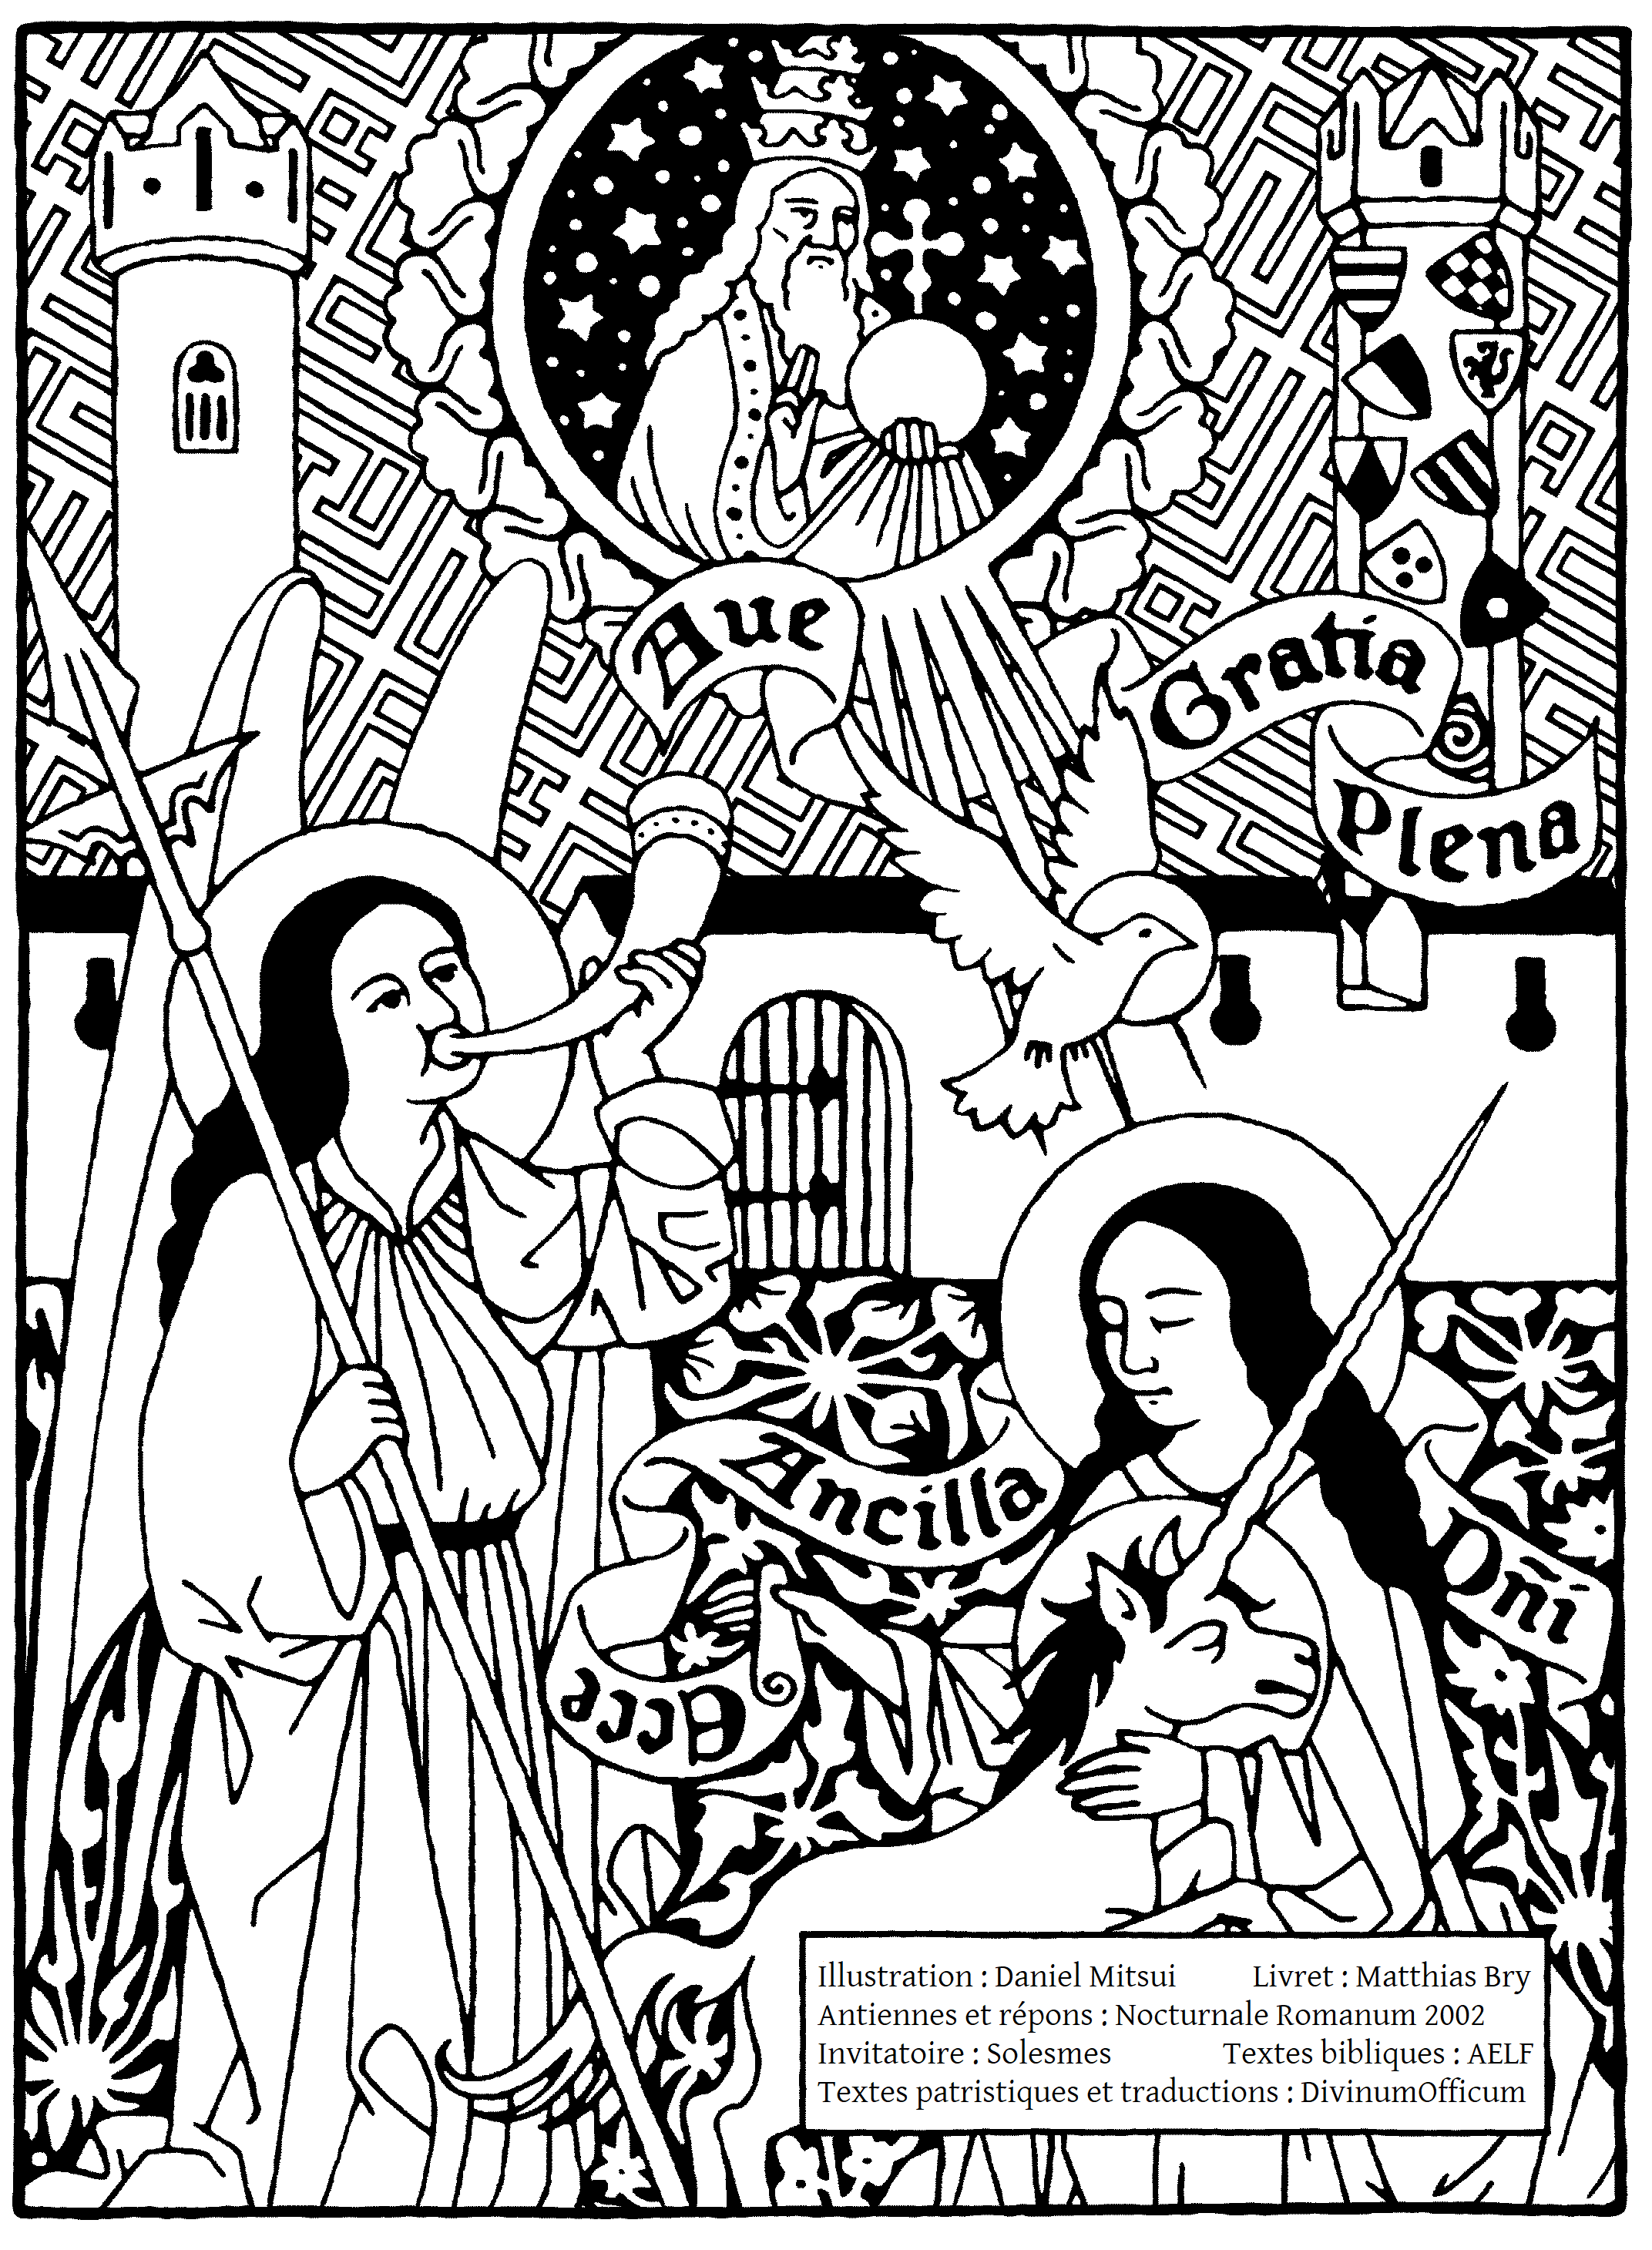
\includegraphics[width=13cm]{4ecouv.png}
\end{adjustwidth}
\end{document} 
